\documentclass[border=4pt]{standalone}
% Shared typography and colours for the standalone figures.
\usepackage{unicode-math}
\setmainfont{TeX Gyre Termes}
\setmathfont{TeX Gyre Termes Math}
\usepackage{tikz}
\usetikzlibrary{arrows.meta,positioning,calc,decorations.pathreplacing}
\usepackage{pgfplots}
\pgfplotsset{compat=1.18}

% One colour per element or subsystem. Record the mapping in
% the working repository conventions and use it identically in every figure.
\definecolor{elemA}{HTML}{1F5FA8}
\definecolor{elemB}{HTML}{B8461B}
\definecolor{elemC}{HTML}{2E7D32}
\definecolor{elemD}{HTML}{6A4C93}
\definecolor{frameline}{HTML}{555555}

% Article-specific diagram styling; common figure-style.tex remains managed.
\usepackage{circuitikz}
\usetikzlibrary{decorations.pathmorphing,fit,backgrounds}
\tikzset{
  every node/.style={font=\small},
  block/.style={draw=frameline,rounded corners=2pt,minimum height=7mm,align=center,fill=white},
  massA/.style={draw=elemA,fill=elemA!10,thick},
  massB/.style={draw=elemB,fill=elemB!10,thick},
  receiver/.style={draw=elemC,fill=elemC!9,thick},
  mediator/.style={draw=elemD,fill=elemD!8,thick},
  flow/.style={-{Latex[length=2.3mm]},thick},
  boundary/.style={draw=frameline,dashed,rounded corners=3pt},
  spring/.style={decorate,decoration={coil,aspect=.4,segment length=3mm,amplitude=1.5mm},thick,elemD}
}

\begin{document}
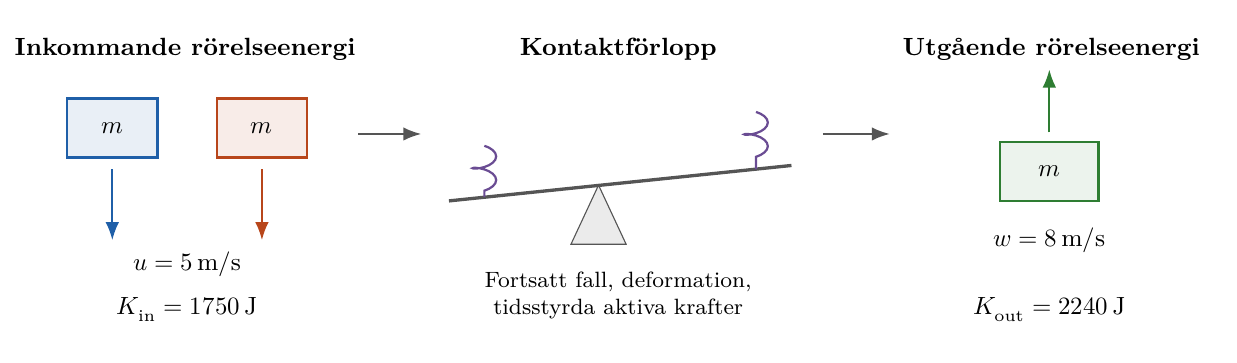
\begin{tikzpicture}
\path[use as bounding box] (0,-.45) rectangle (15,3.45);
\node[font=\small\bfseries] at (2.0,3.18) {Inkommande rörelseenergi};
\node[font=\small\bfseries] at (7.5,3.18) {Kontaktförlopp};
\node[font=\small\bfseries] at (13.0,3.18) {Utgående rörelseenergi};
\draw[massA] (.5,1.8) rectangle (1.65,2.55);
\draw[massB] (2.4,1.8) rectangle (3.55,2.55);
\node at (1.075,2.175) {$m$};
\node at (2.975,2.175) {$m$};
\draw[flow,elemA] (1.075,1.65)--(1.075,.75);
\draw[flow,elemB] (2.975,1.65)--(2.975,.75);
\node at (2.025,.45) {$u=5\,\mathrm{m/s}$};
\node at (2.025,-.13) {$K_{\rm in}=1750\,\mathrm{J}$};
\draw[frameline,very thick] (5.35,1.25)--(9.7,1.7);
\draw[frameline,fill=frameline!12] (7.25,1.45)--(6.9,.7)--(7.6,.7)--cycle;
\draw[spring] (5.8,1.95)--(5.8,1.3);
\draw[spring] (9.25,2.38)--(9.25,1.65);
\draw[flow,frameline] (4.2,2.1)--(5.0,2.1);
\draw[flow,frameline] (10.1,2.1)--(10.95,2.1);
\node[align=center,font=\footnotesize] at (7.5,.05)
 {Fortsatt fall, deformation,\\tidsstyrda aktiva krafter};
\draw[receiver] (12.35,1.25) rectangle (13.6,2.0);
\node at (12.975,1.625) {$m$};
\draw[flow,elemC] (12.975,2.12)--(12.975,2.92);
\node at (12.975,.75) {$w=8\,\mathrm{m/s}$};
\node at (12.975,-.13) {$K_{\rm out}=2240\,\mathrm{J}$};
\end{tikzpicture}
\end{document}
